\begin{exercise}
\label{ex:03-circumbilliard} 
Show that every triangle has a circumbilliard, i.e., an ellipse to which it is inscribed and to which it is a billiard 3-periodic. Compute the axes of said circumbilliard with respect to triangle vertices. 
\end{exercise}
 
\begin{exercise}
 \label{ex:03-power-euler} 
Prove that the power of the circumcircle with with respect to the common center in each of the following 3-periodic families is constant and given by the listed expressions. (i) incircle: $-a_e b_e$; (ii) homothetic: $-({a_e^2+b_e^2})/{2}$, and (iii) excentral: $-a^2-b^2-2\delta$. 
\end{exercise}

%\begin{exercise}\label{ex:33} 
%The {\em cosine circle} (also known as the second Lemoine circle) \cite[Cosine Circle]{mw} of a triangle passes through 6 points: the 3 pairs of intersections of sides with lines drawn through the symmedian $X_6$ parallel to sides of the orthic triangle. Recall that the orthic vertices are the feet of altitudes. Its center is $X_6$ \cite[Cosine Circle]{mw}. If one takes the excentral triangle of a billiard orbit as the reference triangle,   its orthic is the orbit itself.

%Show that the cosine circle of the excentral triangle is invariant over the family of 3-periodic orbits. Its radius $r^*=(a^2-b^2)/\sqrt{2\delta-a^2-b^2}$ is constant and it is concentric and external to the elliptic billiard.
%\end{exercise}

\begin{exercise}
\label{ex:03-cosine-circle}
Prove the radius $r^*$ of the stationary cosine circle of the excentral family is larger than the major axis $a$ of its caustic. 
\end{exercise}

\begin{exercise}
Recall the cosine circle $\Cm$ (also known as the second Lemoine circle) is centered on a triangle's symmedian point $X_6$. Let $\E'$ be the Brocard ellipse of some triangle $T$. Let $\beta$ be the aspect ratio of $\E'$, i.e., $a'/b'$. Show that for any $T$, above (resp. below) a certain $\beta$, $\Cm$ is tangent to $\E'$ at two distinct points (resp. it is exterior to $\E'$). See it \href{https://bit.ly/2RqhUQV}{Live}.
\end{exercise}

\begin{exercise}
Show that over the Brocard porism the radius $r^*$ of the cosine circle is invariant.
\end{exercise}

\begin{exercise}
Show that the first Lemoine circle (centered on $X_{182}$ is stationary over the Brocard porism. Above a certain $a'/b'$, this circle is tangent to one of the minor vertices of the caustic. See it \href{https://bit.ly/3tp0XUq}{Live}.
\end{exercise}

\begin{exercise}
Ehrmann's ``third'' Lemoine circle is studied in \cite{darij2012-ehrmann}, centered on $X_{576}$, is defined as follows: for each vertex, consider the 3 circles containing pairs of vertices and the symmedian point $X_6$. The third Lemoine circle contains the 6 intersections of said circles (2 each) with the sidelines. Prove this circle is also stationary over the Brocard porism, i.e., all three Lemoine circles are; see it \href{https://bit.ly/3tw09gA}{Live}. 
\end{exercise}

\begin{exercise}
Show that over the poristic family, the locus of the foci of the $X_9$-centered circumconic (the circumbilliard) is a circle.
\end{exercise}

\begin{exercise}
Prove \cref{prop:03-antiorthic}. Furthermore, prove the intersection point of $X_1 X_3$ with the antiorthic axis is the Schöder point $X_{1155}$.
\end{exercise}

\begin{exercise}
Prove that over the poristic family the inconic centered on $X_1$ is axis-parallel with the circumconic centered on $X_9$ (i.e., the circumbilliard), see this \href{https://youtu.be/0VHBjdHXbJc}{Video}.
\end{exercise}

\begin{exercise}
A pair of circles uniquely defines a {\em pencil} of coaxial circles; see \cite[Limiting Points]{mw}. The pencil contains exactly two circles which degenerate to a point, known as {\em limiting points}. Derive the location of such points for the poristic pair obtained from the image of two confocal ellipses centered at $[0,0]$ and with axes $a,b$ and $a',b'$.
\end{exercise}

\begin{exercise}
Let $\ell_1,\ell_2$ be the limiting points of the two circles which are polar images of a confocal pair $\E,\E'$ with respect to a circle centered on $f_1$. At what aspect ratio $a/b$ of $\E$ will $\ell_2$ coincide with $f_2$?
\end{exercise}

\begin{exercise}
A well-known result is that the inversion of a circle pair $\Cm,\Cm'$ with respect to a circle $\Cm_1$ centered on $\ell_1$ (resp. $\Cm_2$ centered on $\ell_2$) is a pair of concentric circles $\Cm_1'$ and $\Cm_1''$ (resp. $\Cm_1'$ and $\Cm_1''$). Prove the following lesser known result: the ratio of radii between $\Cm_1'$ and $\Cm_1''$ is the same as the ratio between $\Cm_2'$ and $\Cm_2''$. 
\end{exercise}


\begin{figure}
    \centering
    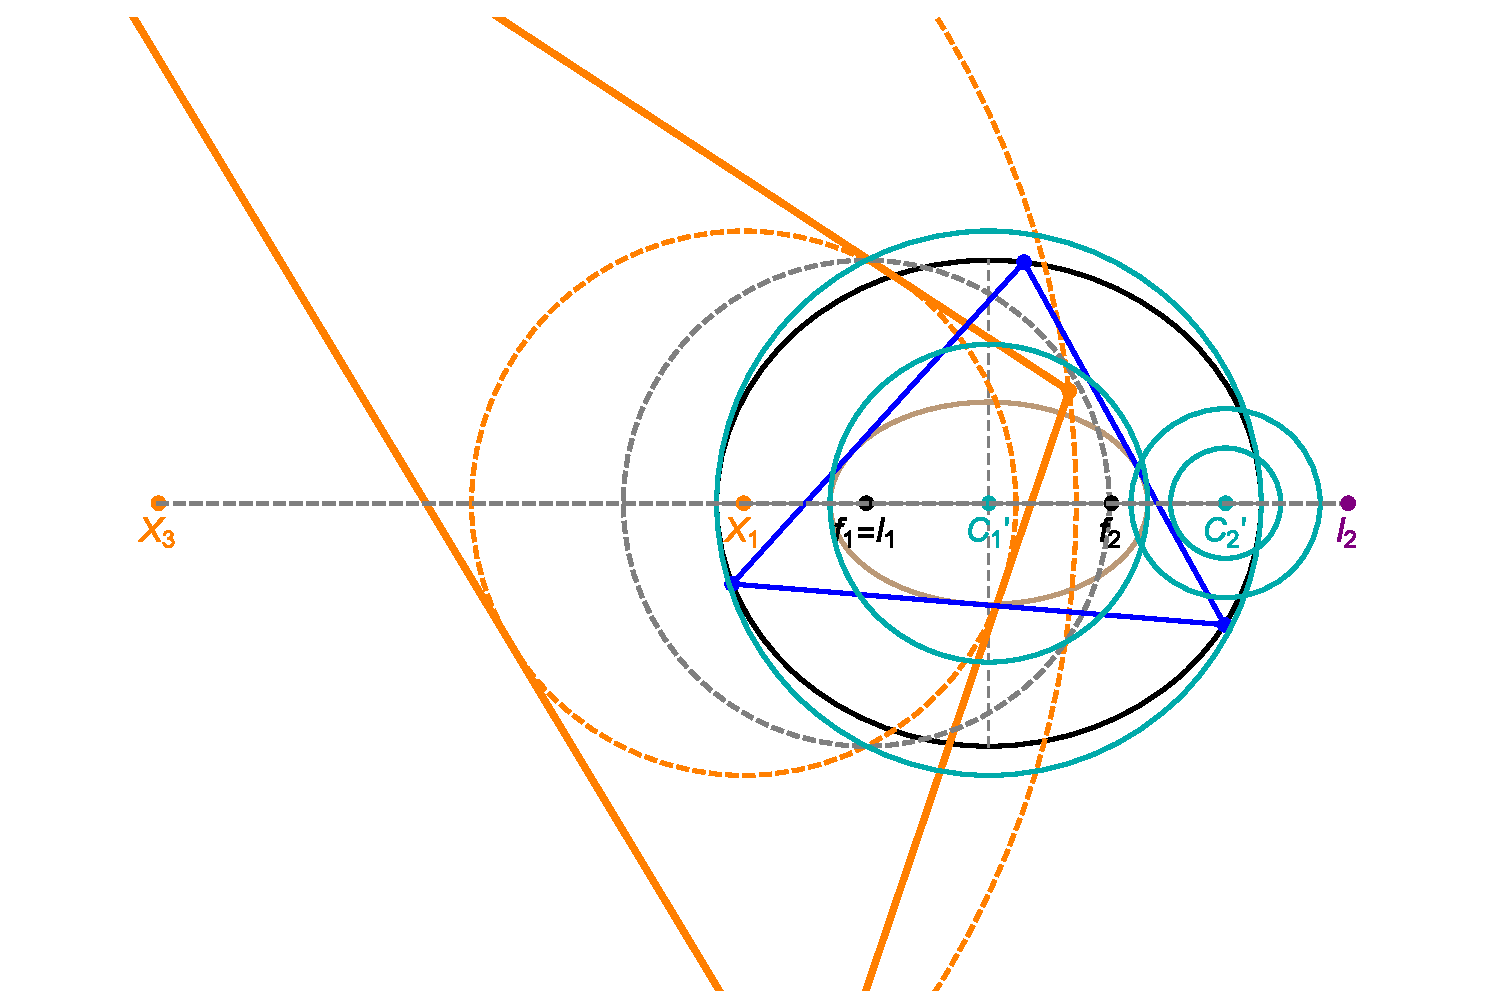
\includegraphics[width=.8\textwidth]{pics_03_210_concentric_inverted_pairs.eps}
    \caption{Concentric circle pairs (light blue) which are the inversions of the circumcircle and incircle (dashed orange) of the bicentric family  (blue) with respect to its two limiting point $\ell_1$ and $\ell_2$. Also shown are Billiard 3-periodics (blue) in the polar pre-image with respect to a circle (dashed gray) -- centered on $f_1=\ell_1$.}
    \label{fig:03-concentric-inverted}
\end{figure}

\begin{exercise}
Referring to \cref{fig:03-concentric-inverted}, let $\Cm,\Cm'$ be the pair of circles which are the polar image of a confocal pair of ellipses $\E,\E'$. Let $\Cm_1', \Cm_1''$ be the inversive images of $\Cm,\Cm'$ wrt to a cirlce centered on a focus of the ellipse pair. Prove that: (i) $\Cm_1'$ and $\Cm_1''$ are concentric with the ellipse pair and (ii) $\Cm_1'$ (resp. $\Cm_1''$) is externally tangent to $\E$ (resp. $\E'$) at its left and right major vertices.
\end{exercise}

\begin{exercise}
Prove \cref{lem:03-circum-x5-locus}.
\label{ex:03-circum-x5-locus}
\end{exercise}

\begin{exercise}
Recall the dual family has stationary orthocenter $X_4$. Prove that the inversive image of the dual family wrt to a circle concentric with the ellipse pair is a non-Ponceletian family with incenter $X_1'$ stationary at the common center. This inversive family is inscribed in Booth's curve and its caustic can contain multiple spikes; see it \href{https://bit.ly/3vCCe05}{Live}.
\end{exercise}

\begin{exercise}
Prove the inversive image of billiard 3-periodics with respect to a focus-centered circle is a non-Ponceletian family inscribed in Pascal's Limaçon whose Gergonne point $X_7$ is stationary; see it \href{https://bit.ly/3edwKD7}{Live}. Indeed, this family has constant perimeter (to be shown later).
\end{exercise}

\begin{exercise}
Show that the poristic excentral family is also the polar image of billiard excentrals wrt to a circle centered on a billiard (i.e., the caustic) focus. See it \href{https://bit.ly/33c1s9A}{Live}.
\end{exercise}

\begin{exercise}
Prove the expression and inequality for $\cot{\omega}$ in \cref{prop:03-brocard-w}.
\end{exercise}

\begin{exercise}
That the Brocard axis $X_3 X_6$ is stationary over the Brocard porism is established. Prove that the Lemoine axis, which intersects the Brocard axis at the Schoutte point $X_{187}$, is also stationary; see it \href{https://bit.ly/3nTRi75}{Live}.
\end{exercise}

\begin{exercise}
The so-called ``second'' Brocard triangle, defined in \cite[Second Brocard Triangle]{mw}, has vertices at the intersections of symmedians (cevians through $X_6$) with the Brocard circle. Show that over the Brocard porism, the family of second Brocard triangles is a new, smaller Brocard porism which shares the isodynamic points $X_{15}$ and $X_{16}$ with the original family. Prove that if this is iterated, the shrinking porisms converge to $X_{15}$. See it \href{https://bit.ly/3ttMNBg}{Live}.
\end{exercise}